\begin{onehalfspace}
\footnotesize
    \noindent A energia elétrica é um recurso essencial para o desenvolvimento econômico de 
    um país, para a qualidade de vida da população e para a manutenção do meio ambiente
    por meio de seu uso eficiente. A importância do uso racional e eficiente deste
    recurso torna imprescindível a conservação e redução do seu desperdício para a 
    sustentabilidade do ambiente em que se vive. Esta gestão eficiente do consumo de energia
    é essencial para reduzir o impacto energético de setores como o de edificações, 
    o qual consome cerca de 36 a 40\% da energia total final no mundo.\vspace*{0.3cm}
    
    \noindent Um exemplo da importância deste recurso e de seu uso devidamente planejado 
    pôde ser observado durante a crise brasileira. Ocorrida em 2001, esta crise provocou 
    mudanças no planejamento do fornecimento de energia elétrica, com o posterior 
    surgimento de medidas atenuantes às dificuldades de cunho ambiental e de 
    infraestrutura da época. Em seu ápice, no ano de 1999, o país passou pelo período 
    popularmente denominado “apagão”, o qual representou a falta de fornecimento 
    em 70\% do território nacional. O consumo de energia elétrica, entre os anos 
    de 1990 e 2000, sofreu aumento de 49\%, enquanto a capacidade instalada foi 
    expandida em 35\%, ocasionando o descompasso entre consumo e fornecimento 
    nesta época.\vspace*{0.3cm}

    \noindent No âmbito estadual, o Espírito Santo vem apresentando redução na produção 
    de energia limpa quando comparado proporcionalmente ao consumo de fontes tradicionais. 
    Existe ainda a parcela de geração de energia elétrica oriunda de fontes não-renováveis 
    de energia, como usinas termelétricas, correspondendo a 65\% de toda a capacidade 
    instalada em operação do Espírito Santo, restando 35\% de fontes renováveis, composta 
    por usinas hidrelétricas, com participação de 34\%, e geradores de energia solar 
    fotovoltaica, com 1\%.\vspace*{0.3cm}

    \noindent Em contraponto à demanda e ineficiência energética, as edificações
    comerciais, em particular as de escritório, podem desempenhar funções estratégicas 
    como minimizar o uso energético e produzir eletricidade, aproximando ou tornando 
    zero a razão entre a produção e o consumo de energia. Estas edificações são 
    denominadas edificações com balanço energético nulo, 
    ou \textit{Zero Energy Buildings} – ZEB.
    Com a introdução de uma ZEB, a exploração de recursos renováveis complementares 
    como a energia solar, e a utilização de tecnologia solar fotovoltaica, surgem como 
    opção para minimizar as consequências negativas causadas por condições climáticas, 
    de infraestrutura e socioeconômicas adversas.\vspace*{0.3cm}

    \noindent A disponibilidade de recursos naturais como a radiação solar recebida 
    no Brasil, por exemplo, concentra grande capacidade de geração de energia solar,
    alcançando a ordem de 1.013 MWh. Este nível de radiação nível acima de países 
    tradicionais na geração de energia fotovoltaica, o que qualidfica a adoção deste 
    recurso como forma de reduzir o uso de fontes de energia fósseis e como economia 
    no consumo de água.\vspace*{0.3cm}

    \noindent Considerando as características do ambiente construído no âmbito da 
    Região Metropolitana da Grande Vitória, é possível desenvolver edificações cujos 
    valores de demanda e produção de energia elétrica resultem em nulo ou quase nulo? 
    Assim, o objetivo principal desta pesquisa foi avaliar a aplicabilidade do conceito 
    \textit{Zero Energy} em edificações comerciais, especificamente de escritório, com 
    o intuito de verificar a validade do método para o cenário construtivo brasileiro 
    adotando como estudo de caso uma edificação fictícia em Vitória (ES).\vspace*{0.3cm}

    \noindent Assim, como ponto de partida, define-se que um edifício 
    \textit{Zero Energy} – ZEB, ou em português, balanço energético nulo, é uma 
    edificação energeticamente eficiente onde, considerada a fonte energética, a 
    energia elétrica fornecida pela concessionária é anualmente menor ou igual à 
    quantidade de energia renovável exportada pela edificação para a rede.\vspace*{0.3cm}

    \noindent Uma outra definição importante iniciada na Europa foi proposta para 
    edificações \textit{Near Net Zero Energy}, nZEB, e em português, próximo ao 
    balanço energético nulo, se apoia na premissa do aproveitamento máximo 
    de recursos para produção de energia, implementando mecanismos à edificação de 
    forma que este aproveitamento aconteça, e a utilização à nível ótimo da energia 
    primária, para um consumo maior que 0 kWh/m² ao ano.\vspace*{0.3cm}

    \noindent Estudos desenvolvidos pela \textit{United Nations Enviroment Programme}
    apontam que 103 países definiram a eficiência energética e uso de energias 
    renováveis como parte importante do seu planejamento estratégico, e destes, 
    79 são países emergentes e em desenvolvimento. Constata-se, ainda, que o 
    consumo de energia poderia ter sido 12\% maior em 2017 caso as políticas 
    públicas mencionadas anteriormente não tivessem sido implementadas desde o ano 2000.\vspace*{0.3cm}

    \noindent 

    \noindent Metodologicamente, este estudo foi desenvolvido com base em três 
    grandes etapas, onde a primeira consistiu em realizar o levantamento das edificações 
    dentro de um recorte territorial pré-estabelecido, selecionar as características 
    construtivas e arquitetônicas mais frequentes entre elas e construir modelos 
    representativos do cenário observado; a segunda consistiu em submeter os modelos
    representativos à simulações computacionais para avaliar o desempenho energético, 
    as possíveis formas de eficientização e de produção de energia; e por fim, a 
    terceira etapa, na qual foi realizada avaliação dos resultados e da viabilidade 
    econômica de implantação do sistema de produção de energia, como representado 
    na Figura \ref{fig:1}.\vspace*{0.3cm}
    \begin{figure}[H]
        \label{fig:1}
        \centering
        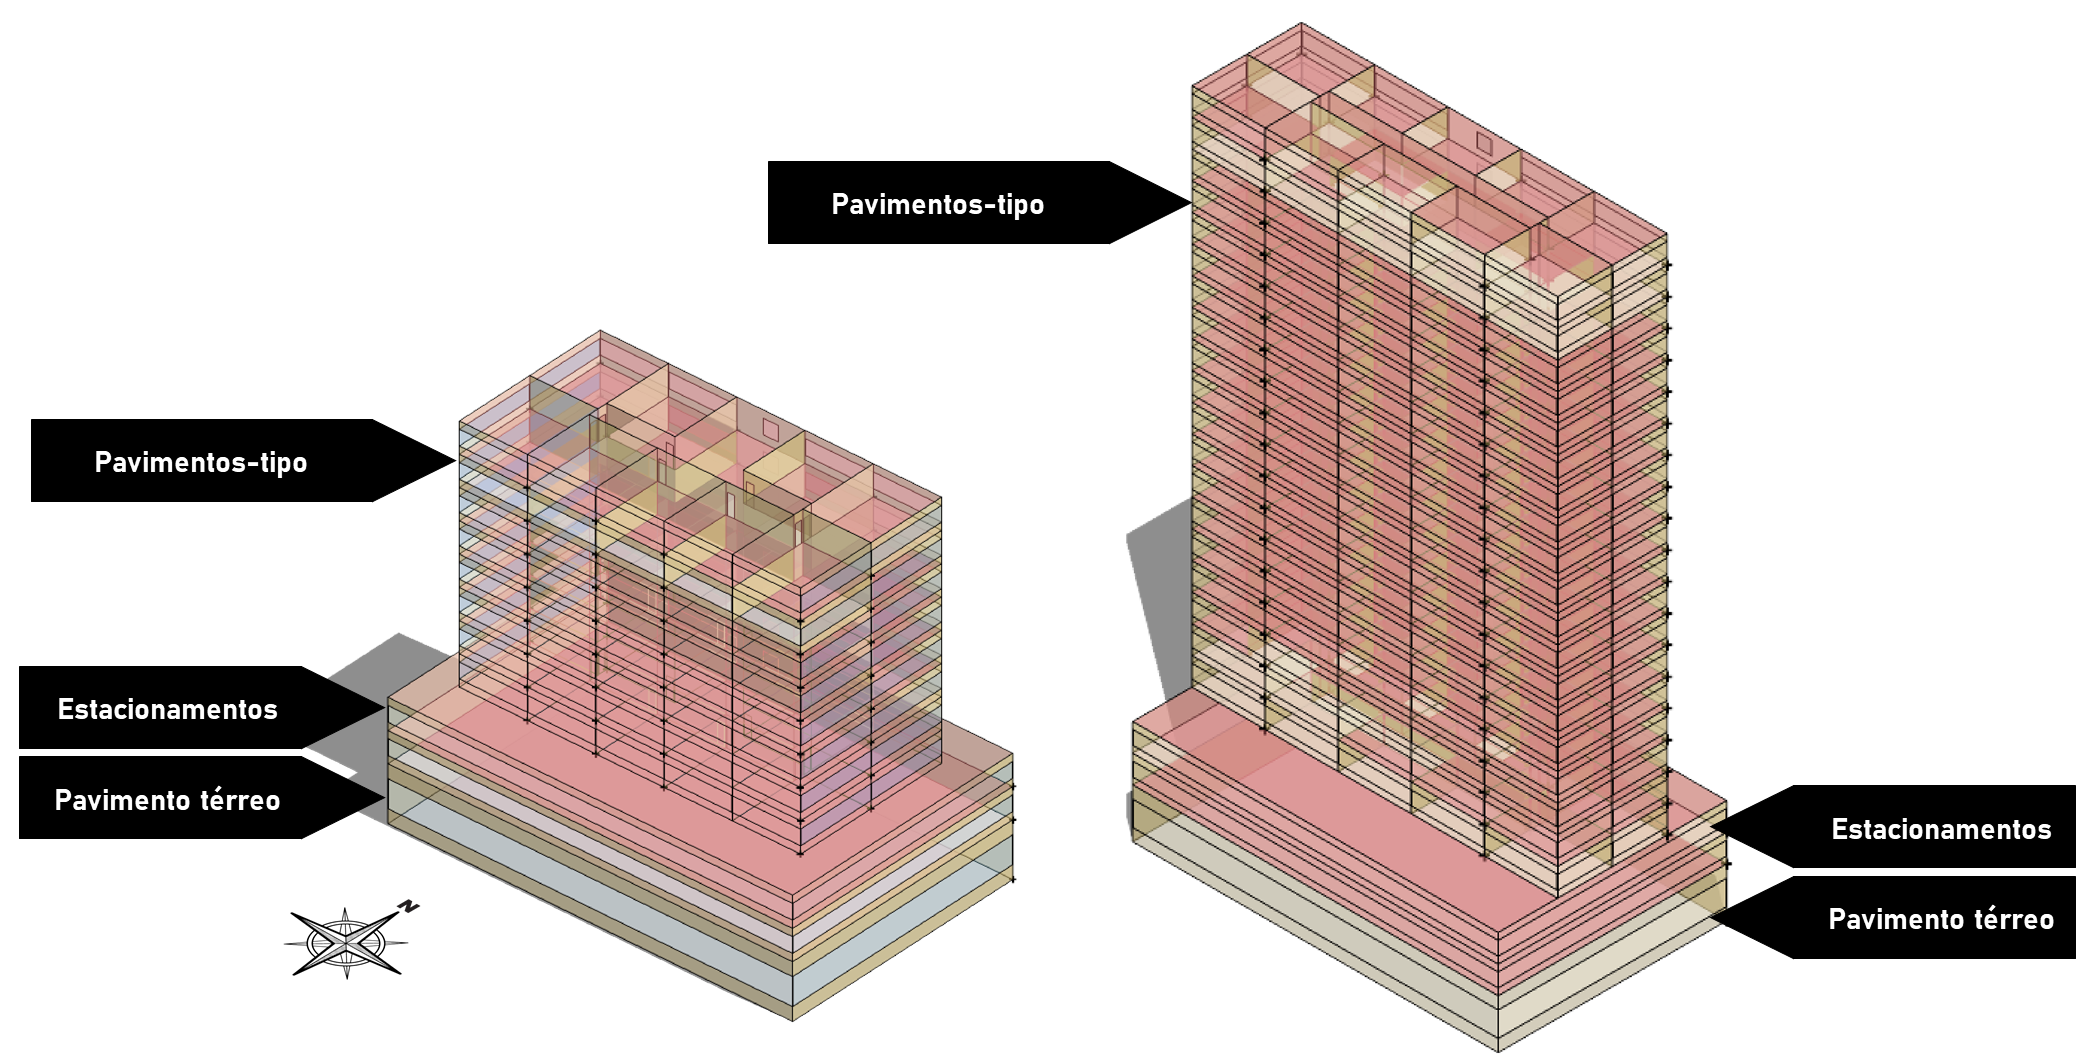
\includegraphics[width=1\textwidth]{figures/fig11_8-19-2pav.png}
        \caption{Fluxograma da avaliação da edificação.}
    \end{figure}
    
    \noindent Os resultados mostraram que as estratégias de implementação de sistemas
    de condicionamento de ar, de equipamentos e iluminação mais eficientes são muito importantes
    para a economia de energia. É perceptível que a proposição de soluções construtivas e
    arquitetônicas mais eficientes em relação ao desempenho energético associado a técnicas de
    obtenção de energia podem resultar em uma edificação com o balanço energético nulo ou
    próximo ao nulo. Esses resultados indicam que a adoção desse conceito para novas edificações é
    factível e cada vez mais acessível à comunidade.\vspace*{0.3cm}
\end{onehalfspace}
